\section{Architektura}

Stroje,
které sestavují či spouštejí aplikace,
nezajímá vzhled či uspořádání zdrojového kódu.
Naopak vývojáři,
jakožto lidé,
potřebují udržovat kód snadno čitelný a srozumitelně rozdělený do jednotlivých
motod, tříd, struktur či vrstev aplikace.
Potřebují také vysokoúrovňové jazyky či pokročilé knihovny a frameworky,
které ulehčí psaní kódu a nenutí vývojáře psát vše odznovu.
I přes to ale nejsou aplikace psány dle nejlepších doporučení
a velmi často vývojáři píší či naráží na tak zvaný \uv{spaghetti code}.
To je mnohdy zapříčeněno nárokem na rychlou implementaci nových funkcí či úprav,
kde vývojáři na úkor času zanedbají čitelnost a strukturu kódu
a čím dál tím více postupem času prohlubují dluh kvality daného kódu.
\cite{architecture}
\todo{\emph{\uv{Software has two types of value:
the value of its behavior and the value of its structure.
The second of these is the greater of the two
because it is this value that makes software soft.}}}
\cite{martin_clean_architecture}
\todo{Jak odkazovat na přímou citaci?}
Dle zmíněného zdroje také plyne,
že se dlouhodobě vyplatí vývoj směřovat k dobré struktuře a architektuře,
než k samotné implementaci,
jelikož implementace se snadno opraví,
kdežto opravit architekturu bez velkého zásahu je značně obtížné.
\cite{martin_clean_architecture}

Cílem každé aplikace je mít udržitelný a snadno rozšiřitelný kód.
Je proto třeba stanovit řadu pravidel,
které pomohou s vývojovými otázkami při návrhu metod, tříd, rozhraní či
celých modulů.
Architektura a její správný a promyšlený návrh umožňuje vyvarovat
se chyb a dluhu ve formě kvality a modularity,
který znemožní snadný proces udržitelnosti aplikace.
\todo{\emph{\uv{Good architecture makes the system easy to understand,
easy to develop, easy to maintain, and easy to deploy.
The ultimate goal is to minimize the lifetime cost of the system
and to maximize programmer productivity.}}}
\cite{martin_clean_architecture}
Dobře navržená a udržovaná architektura tak umožní z dlouhodobého hlediska
produkovat kvalitnější kód.
Kvalitnější architektura tedy logicky minimalizuje nutnost oprav a
přizpůsobení struktury aplikace při vývoji každé nové funkcionality.

Dle zdroje~\cite{architecture} lze rozdělit architektury do dvou skupin:
architektury zaměřené na databázi a architektury zaměřené na doménu.
V následujících sekcích budou popsány rozdíli mezi oběmi skupinami
a vybrané konkrétní případy architektur.

\subsection{Architektury zaměřené na databázi}

Architektury zaměřené na databázi,
také nazývané \emph{database-centric architectures},
byly dle~\cite{architecture} prvním typem softwarových architektur.
Tyto architektury staví databáze do středu dění,
jak jde vidět z obrázku~\ref{fig:architecture_database}.

\begin{figure}
    \centering
    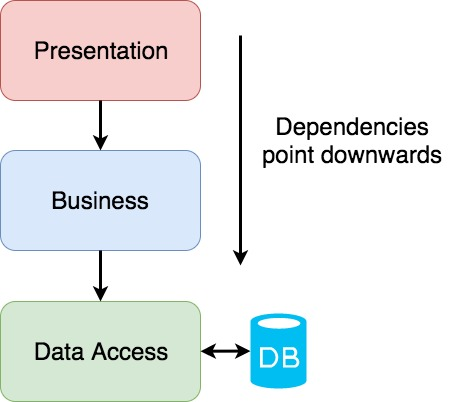
\includegraphics[width=0.5\linewidth]{assets/technology-research/architecture/database-centric.jpg}
    \caption{Schéma architektury zaměřené na databázi \todo{do vektoru}~\cite{architecture}}
    \label{fig:architecture_database}
\end{figure}

Příkladem tohoto typu architektury je tradiční 3-vrstvá architektura.
Ta je robustní a škálovatelná.
Skládá se ze tří vrstev.
První vrstva,
prezentační vrstva,
obsahuje tvorbu UI,
bez samotného kódu s logikou.
Druhá vrstva,
aplikační vrstva,
obsahuje samotné kód s logikou.
Tato vrstva by měla být nezávislá na prezentační vrstvě,
avšak má explicitní závislost na datové vrstvě.
Poslední vrstva,
datová vrstva,
je nejspodnější vrstvou,
která se stará o manipulaci a tok dat z databáze do nižších vrstev.
\cite{architecture}

\begin{listing}
    \caption{Ukázka přístupu zaměřeného na databázi v jazyce Java~\cite{architecture}}
    \label{code:architecture-database}
    \begin{minted}{java}
package ua.com.crosp.testapp.domain;
import ua.com.crosp.testapp.datalayer.PostsRepository;

public class GetRecentPostsUseCase
implements GetRecentPostsUseCaseContract {
    private PostsRepository mPostsRepository;

    public Single<Post.List> execute(Params params) {
        // Execute
    }
}
    \end{minted}
\end{listing}

V této architektuře je největší role přikládána databázi
a často je tak datová a aplikační vrstva úzce propojena.
V nejhorších případech na datové vrstvě závisí i vrstva prezentační.
\cite{architecture}
Ukázka přístupu pomocí této architektury je znázorněna ve výpisu kódu
\ref{code:architecture-database}.

\subsection{Architektury zaměřené na doménu}

\begin{figure}
    \centering
    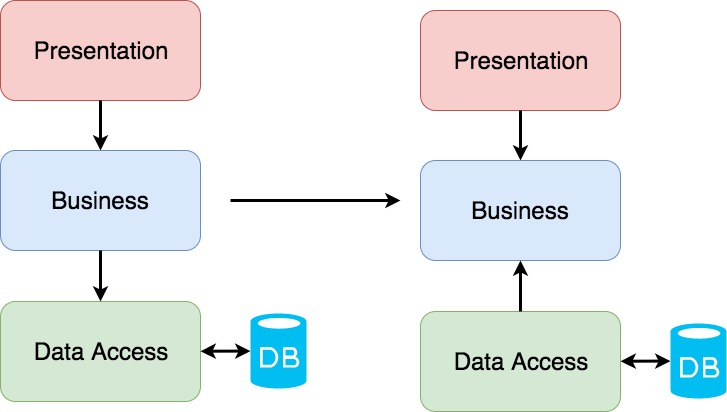
\includegraphics[width=0.5\linewidth]{assets/technology-research/architecture/domain-centric.jpeg}
    \caption{Schéma architektury zaměřené na doménu \todo{do vektoru; oříznout?}~\cite{architecture}}
    \label{fig:architecture_domain}
\end{figure}

Architektury zaměřené na doménu,
také nazývané \emph{domain-centric architectures},
je produktem vývoje z předchozího typu architektur.
Střed dění je přesunut na aplikační vrstvu
--- jak jde vidět z obrázku~\ref{fig:architecture_domain} ---,
protože právě tato vrstva je v aplikaci nejdůležitější,
jelikož se v ní děje implementace nových funkcionalit, změn či oprav.
\cite{architecture}
\todo{\emph{\uv{The way you keep software soft is
to leave as many options open as possible,
for as long as possible.
What are the options that we need to leave open?
They are the details that don’t matter.}}}
\cite{martin_clean_architecture}
Výhodou architektur zaměřených na doménu tedy také je,
že již díky návrhu samotnému abstrahují implementační detaily do podoby
kontraktů.
Těmto kontraktům může nadále vyhovět několik konkrétních implementací,
což umožní snadnou výměnu služeb či jiných závislostí.
\cite{martin_clean_architecture}
Lze tak tedy jednoduše nahradit třeba konkrétní databázi
--- například z databáze MySQL na databázi Cloud Firestore ---,
bez toho,
aniž by se muselo zasahovat do samotné aplikační vrstvy aplikace.
Ukázka přístupu pomocí tohoto typu architektury je znázorněna ve výpisu kódu
\ref{code:architecture-domain}.

\begin{listing}
    \caption{Ukázka přístupu zaměřeného na doménu v jazyce Java~\cite{architecture}}
    \label{code:architecture-domain}
    \begin{minted}{java}
package ua.com.crosp.testapp.domain;
import ua.com.crosp.testapp.domain.PostsRepositoryContract;

public class GetRecentPostsUseCase
implements GetRecentPostsUseCaseContract {
    private PostsRepositoryContract mPostsRepository;

    @Inject
    public GetRecentPostsUseCase(PostsRepositoryContract r) {
        mPostsRepository = r;
    }
    public Single<Post.List> execute(Params params) {
        // Execute
    }
}
    \end{minted}
\end{listing}

\subsection{Clean Architecture}

\todo{Dokončit kapitolu o CA.}

\todo{\emph{\uv{Good software systems begin with clean code.
On the one hand, if the bricks aren’t well made,
the architecture of the building doesn’t matter much.
On the other hand, you can make a substantial mess with well-made bricks.
This is where the SOLID principles come in.}}}~\cite{martin_clean_architecture}

%https://gist.github.com/ygrenzinger/14812a56b9221c9feca0b3621518635b

\todo{Co je Clean Architecture~\cite{martin_clean_architecture}, proč je to fajn používat atp.}
\blind{3}
 
%https://hackernoon.com/hammering-at-clean-architecture-1wbr3cgo

%https://github.com/ResoCoder/flutter-tdd-clean-architecture-course

%https://stackoverflow.com/questions/23479879/clean-architecture-vs-onion-architecture

%TOHLE !! https://crosp.net/blog/software-architecture/clean-architecture-part-2-the-clean-architecture/

%https://blog.cleancoder.com/uncle-bob/2012/08/13/the-clean-architecture.html

%https://github.com/android10/Android-CleanArchitecture

%https://dev.to/bosepchuk/why-i-cant-recommend-clean-architecture-by-robert-c-martin-ofd

%https://proandroiddev.com/clean-architecture-data-flow-dependency-rule-615ffdd79e29

%https://www.freecodecamp.org/news/a-quick-introduction-to-clean-architecture-990c014448d2/

%https://proandroiddev.com/multiple-ways-of-defining-clean-architecture-layers-bbb70afa5d4a

%https://github.com/bufferapp/android-clean-architecture-boilerplate

% https://github.com/bufferapp/android-clean-architecture-boilerplate

\subsection{Zhodnocení}

\todo{Popsat proč si vybírám Clean Architecture.}
\blind{1}
